% =====================================================================================
% CacheGraft -- workshop paper draft
%
% Compile:  pdflatex main && bibtex main && pdflatex main && pdflatex main
%
% To switch to a workshop style file, replace the \documentclass + geometry block with
% the workshop's (neurips_2026.sty / iclr2026_conference.sty / acl.sty) and delete the
% \usepackage{geometry} line. Everything below is style-agnostic.
%
% The system name is defined once as \sys -- change it in one place.
% =====================================================================================
\documentclass[11pt]{article}
\usepackage[margin=1in]{geometry}

\usepackage[T1]{fontenc}
\usepackage[utf8]{inputenc}
\usepackage{microtype}
\usepackage{amsmath,amssymb}
\usepackage{booktabs}
\usepackage{multirow}
\usepackage{graphicx}
\usepackage{xcolor}
\usepackage{url}
\usepackage[numbers,sort&compress]{natbib}
\usepackage[colorlinks=true,allcolors=blue]{hyperref}
\usepackage{tikz}
\usetikzlibrary{arrows.meta,positioning,fit,backgrounds}

\newcommand{\sys}{CacheGraft}
\newcommand{\recv}{\textsc{recv}}
\newcommand{\shr}{\textsc{shr}}
\newcommand{\todo}[1]{\textcolor{red}{\textbf{[TODO: #1]}}}
\newcommand{\best}[1]{\textbf{#1}}

\title{\sys: Precomputed Cross-Model KV Fusion for\\Retrieval-Augmented Generation}

\author{%
  Vihan Lakshman\\
  \texttt{vihanlaks@gmail.com}
  % \todo{affiliation, co-authors}
}
\date{}

\begin{document}
\maketitle

% =====================================================================================
\begin{abstract}
Retrieval-augmented generation (RAG) delivers retrieved context to a language model as
\emph{text}, forcing a small model to encode that context with its own limited parameters.
We ask whether the context can instead be delivered as a \emph{larger model's KV-cache
representation of it}. Building on Cache-to-Cache (C2C) fusion, we show that fusing the
retrieved document only---leaving the query as ordinary text---makes the fused cache
\emph{query-independent}, and therefore precomputable offline. This yields \sys: a two-phase
pipeline in which a large sharer model encodes each corpus passage once, offline, and a small
receiver model decodes every query from the loaded cache with the sharer never running at query
time. On single-hop extractive and knowledge-bottlenecked QA, \sys{} beats the strongest
architecturally-matched baseline---the same small model reading the same passage as text---by
$+8.0$ points on SQuAD and $+5.4$ on TriviaQA under a reference-based LLM judge (paired McNemar
$p<10^{-4}$; the win survives resampling at the passage rather than the question level),
recovering $41\%$ of the receiver-to-sharer quality gap at receiver-only query cost. It also
beats the \emph{cost-matched} offline competitor---the same sharer compressing each passage into
text once, offline---by a \emph{larger} margin ($+10.2$), because the text rungs degrade
monotonically with compression ratio: preprocessing a passage into text is counterproductive
where preprocessing it into KV is worth $+8$. A control that runs the identical cache pipeline
with fusion disabled reproduces the text baseline exactly, isolating the gain to the fused
representation rather than the caching machinery. We also map where the method fails---multi-hop reasoning, chain-of-thought
arithmetic, and questions the receiver already answers parametrically---and unify these
negatives under an \emph{encode/decode} account: KV fusion edits what the receiver can read,
not what it can compute. From that account we derive a four-cell, fuser-free screen that
predicts in advance whether a dataset is fusion-amenable, and validate the pipeline end-to-end
on a second model pair with a fuser we train and release.
\end{abstract}

% =====================================================================================
\section{Introduction}
\label{sec:intro}

Retrieval-augmented generation~\citep{lewis2020rag} has one interface: retrieved passages are
concatenated into the prompt as text. That interface is a bottleneck when the reader is small.
The passage must be re-encoded by the reader's own parameters at every query, so a 0.6B model
reading a dense paragraph recovers only what a 0.6B encoder can recover---and it pays the
prefill cost for those tokens on every query that retrieves them.

Recent systems work attacks the second problem by caching. TurboRAG~\citep{lu2025turborag} and
Prompt Cache~\citep{gim2024promptcache} precompute a passage's KV cache offline and splice it in
at query time; CacheBlend~\citep{yao2025cacheblend} repairs the cross-chunk attention that such
splicing breaks. All of these cache \emph{the reader's own} KV: they change when the encoding
happens, not what the encoding contains.

Cache-to-Cache (C2C) fusion~\citep{c2c2025} suggests the other move. A trained projector maps a
large \emph{sharer} model's KV cache into a small \emph{receiver} model's KV space, so the
receiver attends over keys and values it could not have computed itself. C2C was introduced as
a communication channel between models on a shared prompt. We observe that it is also, and more
usefully, a \emph{RAG} mechanism---and that a specific restriction of it is free at query time.

\paragraph{The observation.} If fusion is applied to the document section of the prompt and
\emph{not} to the question, then, by causality, the fused receiver KV over the document depends
only on the document. It is query-independent. The sharer's encoding of a passage can therefore
be computed once per passage, offline, persisted, and reused for every future query that
retrieves it. At query time only the small receiver runs. We call the resulting system \sys{}
(Figure~\ref{fig:pipeline}).

\paragraph{Contributions.}
\begin{enumerate}\itemsep2pt
\item \textbf{Document-only fusion and its cacheability} (\S\ref{sec:method}). We show that
  section-wise fusion over $[\text{doc}\to\text{fuse},\ \text{question}\to\text{no-fuse}]$ is
  mathematically equivalent to loading an offline-built, question-agnostic fused cache, and we
  implement the offline path as a persisted artifact. The implementations agree to
  $91$--$93\%$ token-exact generations, with the residual attributable to floating-point
  nondeterminism under greedy decoding.
\item \textbf{A win over the baseline that matters} (\S\ref{sec:results}). Against the small
  model reading the same retrieved passage as text---the only architecturally matched
  baseline---\sys{} gains $+8.0$ (SQuAD) and $+5.4$ (TriviaQA) LLM-judge points at top-1
  retrieval, and $+13.7$/$+5.6$ with oracle passages, all paired-significant.
\item \textbf{A complete channel ladder, including the cost-matched text competitor}
  (\S\ref{sec:ladder}). We compare fusion against \emph{three} offline-precomputable text rungs
  at increasing compression. The rungs order monotonically---raw $>$ lightly compressed $>$
  compressed---on every metric and both retrieval settings, so \sys{}'s margin \emph{grows}
  against the more compressed competitor ($+10.2$ / $+17.1$). Compressing a passage into text is
  lossy in a query-agnostic setting; the KV channel is not.
\item \textbf{Causal isolation} (\S\ref{sec:control}). A receiver-own-KV control runs the
  identical two-phase cache pipeline with fusion disabled. It reproduces the text baseline
  ($51.0$ vs $50.4$; $94\%$ token-exact), while \sys{} is $+7.4$ above it. The gain is the fused
  sharer representation, not the plumbing.
\item \textbf{Scope, stated as a mechanism} (\S\ref{sec:scope}). \sys{} does not beat baseline
  on multi-hop HotpotQA, on GSM8K, or on trivia the receiver already knows. We attribute all
  three to the same boundary---fusion edits the KV (read-side), not the output computation
  (decode-side)---and derive a four-cell, fuser-free screen that predicts dataset amenability
  before any training is done.
\item \textbf{A second model pair} (\S\ref{sec:llama}). We train and release a fuser for
  Llama-3.2-1B-Instruct $\leftarrow$ Llama-3.1-8B-Instruct and reproduce the qualitative
  pattern, including the predicted failures.
\end{enumerate}

% =====================================================================================
\section{Background}
\label{sec:background}

\paragraph{Cache-to-Cache fusion.} Given a receiver $\mathcal{M}_\recv$ and a frozen sharer
$\mathcal{M}_\shr$ processing the same token sequence, C2C trains per-layer projectors
$f_\ell$ that map the sharer's cache entries into the receiver's:
$(\tilde K^{\recv}_\ell, \tilde V^{\recv}_\ell) = f_\ell\big((K^{\shr}_{s(\ell)},
V^{\shr}_{s(\ell)}),\ (K^{\recv}_\ell, V^{\recv}_\ell)\big)$, where $s(\cdot)$ is a fixed layer
alignment. Only the projectors are trained; both models stay frozen. Training is general chat
distillation---the released checkpoints never see retrieval data---so every RAG result in this
paper is zero-shot with respect to the fuser's training distribution.

\paragraph{Section-wise application.} Critically for us, the reference implementation applies
fusion \emph{per section} of the prompt rather than per token: the prompt is partitioned into
contiguous sections and each carries a single fuse/no-fuse flag. This is the hook that makes
document-only fusion expressible.

\paragraph{KV caching for RAG.} TurboRAG~\citep{lu2025turborag} precomputes chunk KV caches
offline and rearranges positions at query time; CacheBlend~\citep{yao2025cacheblend}
selectively recomputes high-deviation tokens to restore cross-chunk attention; Prompt
Cache~\citep{gim2024promptcache} reuses modular prompt segments. These reduce prefill cost while
preserving the reader's own representation. \sys{} is orthogonal in what it caches---a
\emph{cross-model} representation---and complementary in mechanism; we use CacheBlend directly
in \S\ref{sec:scope}.

\paragraph{Alternatives to text as the context channel.} Context
compression~\citep{jiang2023llmlingua}, soft-prompt and memory-token methods, and offline
summarization all compress the passage into a shorter or denser input. \sys{} is the opposite
trade: it \emph{expands} storage (a full-length KV tensor) to increase fidelity. We discuss the
resulting storage cost honestly in \S\ref{sec:limitations}.

% =====================================================================================
\section{Method}
\label{sec:method}

\subsection{Document-only fusion}

Let a RAG prompt be the concatenation $x = [p,\ d,\ q]$ of a fixed preamble $p$, a retrieved
document $d$, and a question $q$, followed by generation $g$. \sys{} partitions the prompt into
three sections and assigns fusion flags
\[
\underbrace{[p\,d]}_{\text{fuse}}\ \ \underbrace{[q]}_{\text{no fuse}}\ \ \underbrace{[g]}_{\text{no fuse}} .
\]
The receiver decodes normally; the only difference from vanilla inference is that its cache
entries over $[p,d]$ have been replaced by projected sharer entries.

We contrast this with \emph{full-prompt} fusion ($[p\,d\,q]$ fused), which is C2C's original
setting and which we report as an upper bound (\texttt{doc\_q}). The gap between them is the
\emph{cacheability cost}: what you give up by refusing to let the sharer see the query.

\subsection{Why document-only fusion is precomputable}

\begin{proposition}[Query independence]
\label{prop:cache}
With causal attention and section-wise fusion as above, the receiver's fused cache entries at
positions in $[p,d]$ are a function of $[p,d]$ alone, independent of $q$.
\end{proposition}

\noindent\emph{Argument.} Causal attention makes both models' pre-fusion cache entries at
positions $i \le |p\,d|$ independent of any token at position $j > i$; the projector acts
position-wise and layer-wise on those entries; and the fusion flag for the $[p\,d]$ section is
itself independent of $q$. Hence computing $x=[p,d,q]$ in one forward pass and computing
$[p,d]$ alone yield identical KV over $[p,d]$. $\square$

Two consequences follow. First, the single-pass \texttt{doc\_only} results we report are, by
construction, results for an offline cache---no separate approximation is being measured.
Second, for top-1 retrieval with a fixed preamble, the document always occupies the same
absolute position range, so no RoPE re-rotation is required. Position handling in the style of
TurboRAG becomes necessary only when composing multiple chunks or placing a chunk at a
different offset than it was cached at (\S\ref{sec:scope}).

\subsection{The two-phase pipeline}

\begin{figure}[t]
\centering
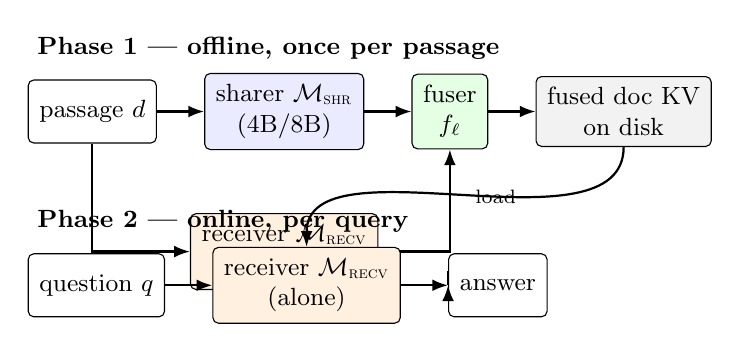
\begin{tikzpicture}[
  node distance=6mm,
  box/.style={draw, rounded corners=2pt, minimum height=8mm, align=center, font=\small, inner sep=4pt},
  big/.style={box, fill=blue!8},
  small/.style={box, fill=orange!12},
  store/.style={box, fill=black!5},
  arr/.style={-{Latex[length=2mm]}, thick}
]
% Phase 1
\node[font=\bfseries\small] (t1) {Phase 1 --- offline, once per passage};
\node[box, below=4mm of t1.west, anchor=north west] (psg) {passage $d$};
\node[big, right=of psg] (sharer) {sharer $\mathcal{M}_\shr$\\(4B/8B)};
\node[small, below=8mm of sharer] (recvA) {receiver $\mathcal{M}_\recv$\\(0.6B/1B)};
\node[box, right=of sharer, fill=green!10] (fuser) {fuser\\$f_\ell$};
\node[store, right=of fuser] (disk) {fused doc KV\\on disk};
\draw[arr] (psg) -- (sharer);
\draw[arr] (psg.south) |- (recvA.west);
\draw[arr] (sharer) -- (fuser);
\draw[arr] (recvA.east) -| (fuser.south);
\draw[arr] (fuser) -- (disk);

% Phase 2
\node[font=\bfseries\small, below=14mm of psg.west, anchor=west] (t2) {Phase 2 --- online, per query};
\node[box, below=4mm of t2.west, anchor=north west] (q) {question $q$};
\node[small, right=of q] (recvB) {receiver $\mathcal{M}_\recv$\\(alone)};
\node[box, right=of recvB] (ans) {answer};
\draw[arr] (q) -- (recvB);
\draw[arr] (ans.west) -- (ans.west);
\draw[arr] (recvB) -- (ans);
\draw[arr] (disk.south) .. controls +(0,-14mm) and +(0,14mm) .. node[right, font=\scriptsize, pos=0.5] {load} (recvB.north);
\end{tikzpicture}
\caption{\sys{}. The sharer and the fuser run only in the offline phase, once per corpus
passage, with no knowledge of any query. At query time the small receiver loads the passage's
fused cache and decodes alone.}
\label{fig:pipeline}
\end{figure}

\paragraph{Phase 1 (offline).} For each corpus passage, prefill $[p,d]$ with fusion enabled and
persist the resulting receiver-space KV, keyed by a content hash of the document section. The
sharer and the projector run here and nowhere else. Cost: $0.1$--$0.2$\,s per $\sim$130-token
passage on an A100, amortized over every future query that retrieves it.

\paragraph{Phase 2 (online).} Load the retrieved passage's cache into the \emph{base} receiver,
prefill the question over it, and greedy-decode. No sharer, no projector, and no sharer-sized
memory on the query path. Cost: $0.52$\,s per query, receiver-only.

% =====================================================================================
\section{Experimental setup}
\label{sec:setup}

\paragraph{Models.} Primary pair: receiver Qwen3-0.6B, sharer Qwen3-4B-Base~\citep{qwen3}, with
the released C2C projector for that pair. Second pair: Llama-3.2-1B-Instruct $\leftarrow$
Llama-3.1-8B-Instruct~\citep{llama3}, with a fuser we train ourselves (\S\ref{sec:llama}).
Greedy decoding, $24$ new tokens, single A100-40GB throughout.

\paragraph{Datasets and retrieval.} \textbf{SQuAD v1.1}~\citep{rajpurkar2016squad}: 500 dev
questions over a pool of 2{,}067 dev paragraphs; gold is the question's own paragraph; top-1
retrieval hit $60.8\%$. Those 500 questions read only $54$ distinct paragraphs
($\approx\!9$ questions per passage). This matters twice over: it is a favourable---and
realistic---reuse rate for an offline-precomputation design, and it means per-question errors
cluster by passage, which we account for in the statistics below.
\textbf{TriviaQA}~\citep{joshi2017triviaqa} (rc.wikipedia): 500 questions
over 21{,}812 $\sim$100-word chunks built from the questions' Wikipedia evidence; a chunk is
gold if it contains an answer alias; top-1 hit $53\%$. \textbf{OpenBookQA}~\citep{mihaylov2018obqa}:
its 1{,}326-fact open book as the retrieval pool; top-1 exact-fact hit $48\%$. Retrieval is
bge-small-en-v1.5~\citep{xiao2023cpack} dense top-1 throughout. We report both
\texttt{retrieved} (realistic) and \texttt{oracle} (perfect-retrieval upper bound) conditions.

\paragraph{Baselines: a ladder of offline-precomputable text channels.} The comparison that
carries the claim is \textbf{receiver text-RAG}: the same receiver, same prompt, same passage,
delivered as text. But that baseline gets no sharer, while \sys{} gets one offline---so we add
the \textbf{cost-matched} competitor, in which the \emph{same} sharer runs once per passage
offline, question-agnostically, and writes \emph{text} instead of a KV tensor. Everything is
held fixed except the channel: same sharer, same once-per-passage offline compute, same
query-agnostic constraint, same receiver decoding alone.

Because a summarizer's aggressiveness is a free parameter, we report two rungs of it rather than
one, so the text channel is beaten at its best rather than its default:
\begin{itemize}\itemsep1pt
\item \textbf{distilled} ($1.7\times$ compression): a 1-shot ``key facts'' completion prompt.
\item \textbf{distilled-strong} ($1.2\times$): a prompt instructing the distiller to preserve
  every name, date, number and title---the spans extractive QA actually asks for.
\end{itemize}
Both use the sharer itself (Qwen3-4B-Base, not an instruct model) so the comparison isolates the
channel and not the model, and both are trimmed to a sentence boundary: at a $96$-token decoding
budget $35\%$ of summaries ended mid-clause, which would have handicapped the baseline for a
decoding reason rather than a channel reason. We additionally report the receiver with no
passage (parametric floor) and the sharer reading the passage as text (quality ceiling).

\paragraph{Metrics.} Our primary metric is a \textbf{reference-based LLM judge}
(Claude Haiku 4.5; pointwise, blind to which system produced the answer, given question,
answer, and gold aliases), scored on the \emph{original} unmodified generations. We use a judge
because the effect interacts with output length: fused generations restate the question with the
answer as a predicate nominal (``The highest mountain in Africa is Kilimanjaro''), which token-EM
and F1 penalize even when correct. We report lexical EM/F1/\texttt{contains} as a secondary
family, computed after a \emph{uniform} answer-extraction post-process applied identically to
every system. Significance is exact two-sided paired McNemar over per-question correctness.
Because SQuAD questions cluster heavily by passage, we additionally report a \textbf{cluster
bootstrap} that resamples \emph{passages} rather than questions---the honest unit of analysis for
this design, and a strictly more conservative test than McNemar.

% =====================================================================================
\section{Results}
\label{sec:results}

\subsection{Main result}

\begin{table}[t]
\centering
\small
\caption{Main result, Qwen3-0.6B receiver $\leftarrow$ Qwen3-4B-Base sharer, top-1 retrieval,
$n\!\approx\!500$. LLM-judge accuracy (\%). \sys{} is the cacheable \texttt{doc\_only} setting:
the sharer never runs at query time. $\Delta$ and McNemar are against receiver text-RAG.}
\label{tab:main}
\begin{tabular}{lcccc}
\toprule
 & \multicolumn{2}{c}{\textbf{SQuAD}} & \multicolumn{2}{c}{\textbf{TriviaQA}} \\
\cmidrule(lr){2-3}\cmidrule(lr){4-5}
System & retrieved & oracle & retrieved & oracle \\
\midrule
Receiver only, no passage        & $\approx 0$ & --- & 17.0 & --- \\
Receiver text-RAG \emph{(baseline)} & 50.4 & 70.4 & 37.6 & 52.6 \\
\quad + offline sharer distillation \emph{(cost-matched)} & 48.2 & 66.9 & --- & --- \\
Receiver-own-KV control (\S\ref{sec:control}) & 51.0 & 69.0 & --- & --- \\
\textbf{\sys{} (doc-only fusion)}   & \best{58.4} & \best{84.1} & \best{43.0} & \best{58.2} \\
\quad\emph{persisted-cache implementation} & 57.2 & 83.4 & 43.6 & 57.4 \\
\midrule
$\Delta$ vs.\ baseline & $+8.0$ & $+13.7$ & $+5.4$ & $+5.6$ \\
McNemar (win/lose, $p$) & 63/24, $<$.0001 & 94/27, $<$.0001 & 52/25, .0028 & 58/30, .0037 \\
Passage-cluster 95\% CI & [+2.7,\,+14.1] & [+7.5,\,+19.9] & --- & --- \\
\midrule
Sharer text-RAG \emph{(ceiling)} & 70.0 & --- & --- & --- \\
\bottomrule
\end{tabular}
\end{table}

Table~\ref{tab:main} is the headline. Delivering the retrieved passage as the sharer's projected
KV rather than as text improves the small receiver by $+8.0$ points on SQuAD and $+5.4$ on
TriviaQA at realistic top-1 retrieval, with larger gains under oracle retrieval. On SQuAD the
receiver-to-sharer gap is $50.4 \to 70.0$; \sys{} closes $41\%$ of it while paying only
receiver-sized cost at query time. The gain is not an artifact of treating clustered questions as
independent: resampling the $53$ distinct retrieved passages leaves the confidence interval
clear of zero in both settings ($p_{\text{clu}}\!\le\!0.001$).

\paragraph{Cacheability is nearly free.} Full-prompt fusion (\texttt{doc\_q}), where the sharer
also sees the question, is an upper bound on what fusion can deliver. On TriviaQA lexical
metrics it exceeds \texttt{doc\_only} by only $0$--$0.6$ EM and $1.6$--$2.4$ F1
(Table~\ref{tab:lexical}). Refusing the sharer any knowledge of the query---the entire basis of
offline precomputation---costs remarkably little.

\paragraph{Fusion also beats text on OpenBookQA.} With no retrieval at all, fusing the question
lifts the receiver from $39.6$ to $53.4$ accuracy (reproducing C2C's reported result). With
top-1 retrieval of a science fact, text-RAG reaches $46.2$ and \sys{} reaches $62.2$; with the
gold fact, $56.4$ vs $69.0$. Fusion beats text at identical retrieval by $+16$ points.

\subsection{The channel ladder: text compression is lossy, KV is not}
\label{sec:ladder}

\begin{table}[t]
\centering
\small
\caption{The offline-precomputable channel ladder on SQuAD (LLM judge, $n{=}490$). Every rung
below the first runs the \emph{same} sharer once per passage, offline and question-agnostically;
they differ only in what gets written down. Text quality falls monotonically with compression,
so \sys{}'s margin is \emph{largest} against the most compressed competitor.}
\label{tab:ladder}
\begin{tabular}{llccc}
\toprule
Channel & stored/passage & retrieved & oracle & $\Delta$ vs.\ \sys{} \\
\midrule
\textbf{\sys{}} (fused KV) & $\sim$18\,MB & \best{58.4} & \best{84.1} & --- \\
\midrule
raw passage ($1.0\times$) & $\sim$0.7\,kB & 50.4 & 70.4 & $-8.0$ / $-13.7$ \\
distilled-strong ($1.2\times$) & $\sim$0.6\,kB & 48.2 & 66.9 & $-10.2$ / $-17.1$ \\
distilled ($1.7\times$) & $\sim$0.4\,kB & 40.4 & 53.3 & $-18.0$ / $-30.8$ \\
\bottomrule
\end{tabular}
\end{table}

\begin{table}[t]
\centering
\small
\caption{Paired significance for Table~\ref{tab:ladder}. McNemar is exact two-sided over
questions; the cluster interval resamples the $53$ distinct passages.}
\label{tab:ladder_sig}
\begin{tabular}{llcccc}
\toprule
\sys{} vs. & setting & $\Delta$ & win/lose & McNemar $p$ & passage-cluster 95\% CI \\
\midrule
raw passage      & retrieved & $+8.0$  & 63/24  & $<10^{-4}$ & [+2.7,\ +14.1] \\
distilled-strong & retrieved & $+10.2$ & 74/24  & $<10^{-4}$ & [+3.7,\ +17.8] \\
distilled        & retrieved & $+18.0$ & 106/18 & $<10^{-4}$ & [+9.9,\ +27.5] \\
raw passage      & oracle    & $+13.7$ & 94/27  & $<10^{-4}$ & [+7.5,\ +19.9] \\
distilled-strong & oracle    & $+17.1$ & 115/31 & $<10^{-4}$ & [+10.3,\ +24.8] \\
distilled        & oracle    & $+30.8$ & 177/26 & $<10^{-4}$ & [+23.8,\ +38.5] \\
\bottomrule
\end{tabular}
\end{table}

The objection Table~\ref{tab:main} invites is that \sys{} is handed a 4B model and the text
baseline is not. Table~\ref{tab:ladder} answers it by giving the text channel the same 4B, used
the same way---once per passage, offline, without seeing the question---and letting it write text
instead of a tensor.

The result is not the one we expected. The distilled rungs do not close the gap; they fall
\emph{below} raw text, and they do so monotonically in the compression ratio, on every metric and
in both retrieval settings (Table~\ref{tab:lexical_squad}). The mechanism is visible in the data:
a query-agnostic summary must serve every future question about its passage---here about nine of
them---so any compression is compression against an unknown query, and reliably discards the span
some future question wanted. The $1.2\times$ rung recovers most of the loss precisely by
declining to compress.

Two conclusions follow, and the second is stronger than the one we set out to defend.
\textbf{First}, raw text remains the binding baseline: since the distilled rungs sit below it,
Table~\ref{tab:main}'s comparison is the conservative one. \textbf{Second}, offline sharer
compute spent on \emph{text} is counterproductive on this task, while the same compute spent on
\emph{KV} is worth $+8$ to $+13.7$. The interesting quantity is therefore not whether fusion
beats summarization but why the two directions have opposite signs, which is exactly the
information-bottleneck claim: text is a low-bandwidth serialization that the receiver must
re-encode with its own parameters, whereas the fused cache is a function of the passage the
receiver \emph{cannot compute at any length}.

We report this as a measured trade rather than a free win. The KV channel buys those points at
roughly $2.6\times10^{4}$ times the storage of the passage text (\S\ref{sec:limitations}).

\subsection{The gain is the fused representation, not the cache pipeline}
\label{sec:control}

The most likely alternative explanation for Table~\ref{tab:main} is that our two-phase pipeline
differs from batched text inference in some incidental way---prefill chunking, section
boundaries, the manual decode loop. We test it directly: run the \emph{identical} pipeline,
build the document cache from the receiver's \emph{own} KV (fusion flag off), and change nothing
else.

The control lands on the text baseline: $51.0$ vs $50.4$ (retrieved) and $69.0$ vs $70.4$
(oracle), with $94\%$ token-exact agreement with text-RAG generations. Against the same
pipeline with fusion \emph{on}, \sys{} is $+7.4$ (retrieved, $p=0.0002$) and $+14.7$ (oracle,
$p<0.0001$). Within-pipeline, the only variable is whose KV fills the document section, and it
accounts for the entire effect.
\todo{the receiver-own-KV cells, the persisted-cache cells and the sharer ceiling are carried
over from an earlier run; re-run them so every number in the paper comes from one environment.
The text/fusion/distilled cells in Tables~\ref{tab:main}--\ref{tab:ladder_sig} are from the
current run.}

\subsection{Lexical metrics and the verbosity confound}

\begin{table}[t]
\centering
\small
\caption{TriviaQA lexical metrics ($n=500$, matched short-answer protocol and uniform answer
extraction on both channels). \texttt{doc\_q} is the non-cacheable upper bound.}
\label{tab:lexical}
\begin{tabular}{lcccccc}
\toprule
 & \multicolumn{3}{c}{\textbf{retrieved}} & \multicolumn{3}{c}{\textbf{oracle}} \\
\cmidrule(lr){2-4}\cmidrule(lr){5-7}
System & EM & F1 & contains & EM & F1 & contains \\
\midrule
Receiver, no passage & 8.2 & 15.5 & 15.6 & --- & --- & --- \\
Sharer, no passage & 5.4 & 24.8 & 34.4 & --- & --- & --- \\
Receiver text-RAG & 25.0 & 33.4 & 33.4 & 35.2 & 43.9 & 45.8 \\
\textbf{\sys{} (doc\_only)} & \best{29.2} & \best{37.3} & \best{39.2} & \best{41.8} & \best{50.9} & \best{55.8} \\
\quad full-prompt fusion (doc\_q) & 29.8 & 39.7 & 44.4 & 41.8 & 52.5 & 60.8 \\
\bottomrule
\end{tabular}
\end{table}

\begin{table}[t]
\centering
\small
\caption{SQuAD lexical metrics ($n{=}500$, original prompts, uniform answer extraction). The
text rungs order monotonically with compression on \emph{every} metric. \sys{} wins
\texttt{contains} decisively and loses EM to verbosity---the split the judge resolves.}
\label{tab:lexical_squad}
\begin{tabular}{lcccc}
\toprule
System & EM & F1 & contains & words \\
\midrule
\multicolumn{5}{l}{\emph{retrieved}} \\
\quad\textbf{\sys{} (doc\_only)} & 21.0 & 35.4 & \best{55.6} & 7.3 \\
\quad receiver text-RAG (raw) & \best{30.8} & \best{41.7} & 50.8 & 4.4 \\
\quad distilled-strong ($1.2\times$) & 29.4 & 39.3 & 47.6 & 4.5 \\
\quad distilled ($1.7\times$) & 23.4 & 33.1 & 40.2 & 4.6 \\
\midrule
\multicolumn{5}{l}{\emph{oracle}} \\
\quad\textbf{\sys{} (doc\_only)} & 30.8 & 49.8 & \best{78.4} & 6.7 \\
\quad receiver text-RAG (raw) & \best{43.2} & \best{56.7} & 69.0 & 3.9 \\
\quad distilled-strong ($1.2\times$) & 42.4 & 54.1 & 64.6 & 4.0 \\
\quad distilled ($1.7\times$) & 31.8 & 43.1 & 51.6 & 4.2 \\
\bottomrule
\end{tabular}
\end{table}

Fused generations are systematically wordier than text-RAG generations, because fusion changes
what the receiver can \emph{read} without changing its output habits. Under a matched
short-answer protocol and a uniform extraction rule applied to every system, \sys{} wins EM, F1
and \texttt{contains} on TriviaQA (Table~\ref{tab:lexical}; McNemar $p \le .026$ on EM, $p \le
.002$ on \texttt{contains}).

On SQuAD, under the original prompts, the two families split (Table~\ref{tab:lexical_squad}):
\sys{} wins \texttt{contains} by $+4.8$ (retrieved) and $+9.4$ (oracle) while losing EM by
$-9.8$/$-12.4$, at $7.3$ versus $4.4$ words. This is the encode/decode signature---fusion lifts
what is \emph{accessible} far more than it changes \emph{how the receiver writes}---and it is
why the judge is our primary metric.

\paragraph{The win does not depend on the judge; only its size does.} It is worth separating the
two. On \texttt{contains}, a metric with no model in the loop, \sys{} already leads by $+6.2$
(retrieved) and $+11.2$ (oracle). EM is the sole metric on which it loses, and that loss is
verbosity. So the judge is not manufacturing the result---it is adjudicating its magnitude.

\paragraph{Bounding judge bias.} The judge's plausible failure mode points in the same direction
as the effect: a length-tolerant grader would flatter the wordier system. We can bound it. The
judge's net correction over \texttt{contains} is $+1.8$ points for \sys{} versus $+0.2$ for raw
text (retrieved), and $+3.4$ versus $+1.2$ (oracle)---differentials of $1.6$ and $2.2$.
Attributing the \emph{entire} differential to length bias still leaves $+6.4$ and $+11.5$. The
conclusion therefore survives a total-bias assumption, which is a stronger guarantee than a spot
check; we nonetheless regard human-labelled validation as required work (\S\ref{sec:limitations}).

\subsection{Cost}

Phase 1 costs $0.1$--$0.2$\,s and $\sim$18\,MB (fp16) per $\sim$130-token passage, incurred once
per passage regardless of how many queries later retrieve it. Phase 2 costs $0.52$\,s per query
with only the receiver resident. At our scale ($n{=}500$ unique passages, 24 decode steps) the
per-query wall-clock win is modest because decoding dominates; the structural wins are that (i)
the sharer leaves the query-time critical path \emph{and memory}, and (ii) offline cost amortizes
with passage reuse. Both grow with sharer size, passage length, and reuse rate. The storage
figure is a real cost, not a rounding error, and we treat it as such in \S\ref{sec:limitations}.

% =====================================================================================
\section{Where fusion helps, and why}
\label{sec:scope}

\subsection{Three negatives with one explanation}

\sys{} does not win everywhere, and the failures are informative.

\textbf{GSM8K (chain-of-thought arithmetic).} Fused RAG scores $\sim$30 against the receiver's
own $54.7$ zero-shot---worse than doing nothing. \textbf{HotpotQA (multi-hop).} With top-$k$
retrieval, the cacheable configuration does not beat the receiver reading the passages as text.
\textbf{TriviaQA on the Llama pair.} $-1.8$ points, not significant, despite a very large
sharer-receiver quality gap.

We attribute all three to one boundary. \emph{Fusion edits the KV cache---the read side---not
the output computation.} It changes what content is accessible to attention; it cannot supply a
computation the receiver must perform at decode time. Multi-step arithmetic and cross-passage
linking are decode-time computations. So, we argue, is open-domain parametric recall: on
TriviaQA the 8B sharer's advantage is parametric, not document-derived (8B with no passage,
$73.6$ \texttt{contains}, $\approx$ 8B reading the passage, $72.0$), and correspondingly fusing
the sharer's encoding of the \emph{question} \emph{hurts} the receiver ($44.2 \to 36.2$)---the
answer materializes in the sharer's decode, and there is no KV to transfer it in.

This account also predicts the positive results: OpenBookQA and SQuAD are exactly the cases
where the answer is present in the retrieved text and the receiver under-encodes it.

\subsection{A fuser-free amenability screen}

The account yields a cheap pre-experiment. Fusion should help only when \emph{both}:
\[
\underbrace{\text{sharer-text} - \text{receiver-text}}_{\text{encoding headroom}} \gg 0
\qquad\text{and}\qquad
\underbrace{\text{sharer-text} - \text{sharer-no-passage}}_{\text{answer-in-document}} \gg 0 .
\]
Both are measurable with four batched inference cells and \emph{no fuser}---before committing to
any training run. The second cell doubles as a pretraining-contamination detector.

\begin{table}[t]
\centering
\small
\caption{Amenability screen (F1, oracle context, $n=500$, Llama pair). Fusion requires both
columns on the right to be large. TriviaQA, where fusion failed, flunks the answer-in-document
precondition.}
\label{tab:screen}
\begin{tabular}{lcccc|cc}
\toprule
Dataset & 1B-none & 8B-none & 1B-text & 8B-text & enc.\ headroom & answer-in-doc \\
\midrule
NarrativeQA & .05 & .07 & .53 & .69 & $+0.15$ & \best{$+0.62$} \\
PubMedQA & .26 & .55 & .44 & .66 & $+0.22$ & $+0.11$ \\
BoolQ & .22 & .66 & .35 & .81 & $+0.46^{*}$ & $+0.15$ \\
TriviaQA \emph{(fusion failed)} & .39 & .72 & .63 & .81 & $+0.18$ & $+0.09$ \\
\bottomrule
\end{tabular}
\\[2pt]
\footnotesize{$^{*}$inflated by the yes/no format---the 1B rarely emits a clean label.}
\end{table}

Table~\ref{tab:screen} shows the screen separating datasets in the predicted direction. It also
sharpens where we think this method belongs: public Wikipedia-derived RAG benchmarks largely test
facts the models already hold parametrically, which is the \emph{worst} case for fusion. The
preconditions operationalize the good case---non-parametric, hard-to-encode corpora---which is
also where offline precomputation pays off most (private and enterprise corpora, high passage
reuse, no query-time budget for a large model). The architecture and the accuracy precondition
point at the same deployment.

\paragraph{A falsifiable prediction.} The current general-chat fuser captures none of
NarrativeQA's headroom (doc-only F1 $0.437$ vs the $0.534$ text bar). Because the headroom there
is \emph{reachable} in principle (answer in document), we predict that RAG-aware fuser training
flips NarrativeQA to a win but does \emph{not} fix TriviaQA, whose deficit is structural. We
have not run this yet; it is the cleanest available test of the encode/decode account.

\subsection{Multi-chunk composition}

Extending to top-$k$ forces composing independently-cached chunks. We find (i) most of the
multi-document loss is RoPE \emph{position gaps} rather than lost cross-chunk attention---with
dense contiguous placement, block-local composition is roughly flat on single-hop SQuAD; (ii) on
multi-hop HotpotQA cross-chunk attention genuinely matters (full attention improves with $k$
while block-local declines, a $+10.7$ gap at $k{=}4$); and (iii)
CacheBlend~\citep{yao2025cacheblend}, recomputing the top-15\% highest-deviation tokens, recovers
$56$--$111\%$ (receiver) and $33$--$47\%$ (fused) of that gap training-free. The mechanism works;
it does not overturn the multi-hop baseline, consistent with \S\ref{sec:scope}. A structural
obstacle remains: fused keys are not RoPE-re-rotatable, so a single canonical cached copy cannot
serve arbitrary slots. We return to this in \S\ref{sec:limitations}.

% =====================================================================================
\section{A second model pair, with a fuser we train}
\label{sec:llama}

The released projectors are Qwen-only, so reproducing the pipeline on a new pair requires
training one. We train a fuser for Llama-3.2-1B-Instruct $\leftarrow$ Llama-3.1-8B-Instruct
(16 projectors, 268M trainable parameters, 2.8\% of the receiver-side stack; shared Llama-3
vocabulary, so no token alignment is needed) on 150k OpenHermes-2.5 chat samples---general
dialogue, \emph{no} retrieval data---for one epoch on a single A100-40GB ($\sim$12.5\,h). Every
RAG number below is therefore zero-shot with respect to fuser training.

Results reproduce the qualitative picture and its boundary: OpenBookQA $27.6 \to 40.8$ with pure
fusion and $41.2 \to 47.8$ over text-RAG; SQuAD $57.3 \to 61.2$ judge ($p{=}0.042$); TriviaQA
$52.0 \to 50.2$, not significant---the predicted failure. Notably, scaling training from 50k to
150k samples \emph{flipped} SQuAD doc-only from $-1.0$ (n.s.) to $+3.9$ ($p{=}0.042$) while
eval loss fell $0.879 \to 0.717$: the cacheable projection is the harder one to learn and is
the first to benefit from more data. We are still an order of magnitude below the released
fusers' training budget, so these gains should be read as a lower bound. The checkpoint and
recipe are released.

Two caveats. The absolute gains are smaller than with the Qwen pair, and the SQuAD gain is
smaller than the Qwen pair's $+8.0$ despite a \emph{larger} sharer-receiver gap. Our reading is
that Llama-3.2-1B-Instruct is already a competent extractive reader (text-RAG judge $57.6$ vs
Qwen-0.6B's $50.4$), leaving less encoding deficit to fill. That is a prediction about scaling
that cuts against the method, and we state it as such: the benefit should shrink as receivers
get stronger. Testing it at 7B-receiver scale is the most important open question about the
method's reach (\S\ref{sec:limitations}).

% =====================================================================================
\section{Limitations}
\label{sec:limitations}

\paragraph{Storage---the central cost.} A fused cache is $\sim$18\,MB per $\sim$130-token
passage in fp16, roughly $2.6\times10^{4}$ times the passage's text. A million-passage corpus
would be $\sim$18\,TB. \S\ref{sec:ladder} establishes that the cheap text alternatives are
\emph{worse}, not merely cheaper, so the trade is real rather than dominated---but it is a trade,
and we have not yet measured KV quantization or head-pruning to reduce it, nor characterized the
reuse rate at which precomputation pays for itself. We note that our SQuAD setting already has a
favourable reuse rate ($\approx\!9$ queries per cached passage), which a corpus with a long tail
of rarely-retrieved documents would not.

\paragraph{Judge validation.} The primary metric is an LLM judge, and the measured effect is
entangled with output length in exactly the direction a length-tolerant judge would inflate. We
bound that exposure in \S\ref{sec:results}---the conclusion survives attributing the entire
differential correction to bias---and we note that \sys{} already leads on \texttt{contains},
which involves no model judgement at all. What we have \emph{not} done is measure per-system
judge error against human labels or replicate with a second judge family. Until both are done,
treat the exact magnitudes as provisional and the sign as robust.

\paragraph{Scale and scope.} All results use 0.6B/1B receivers, top-1 (or small-$k$) retrieval,
$n{=}500$ per cell, greedy decoding, and clean topically-focused retrieval pools. We do not know
whether the effect survives stronger receivers, adversarial or off-topic retrieval, or corpora
with millions of distractors. The short-answer extraction rule was tuned on the same data it is
evaluated on; the LLM-judge results, computed on unmodified generations, are not subject to that
concern.

\paragraph{Multi-chunk.} Fused keys are not RoPE-re-rotatable, so top-$k$ composition currently
requires caching per (chunk, slot) pair. A position-decoupled projector would remove this and is
the most promising architectural direction we see.

% =====================================================================================
\section{Conclusion}

Retrieved context does not have to reach a small model as text. If a larger model's KV encoding
of a passage is fused in for the document section only, the encoding is query-independent, can
be computed once offline, and improves the small model's answers over reading the same passage
itself---by $+8.0$ (SQuAD) and $+5.4$ (TriviaQA) judge points at receiver-only query cost, with
the gain isolated to the fused representation by a within-pipeline control. Spending the same
offline budget on \emph{text} instead does not merely underperform fusion, it underperforms
doing nothing at all: query-agnostic summaries lose quality monotonically with compression,
because they must be written before the query is known. The method is a
knowledge-injection mechanism, not a reasoning one: it fails on multi-hop, on chain-of-thought,
and on questions answered from the sharer's parameters rather than the document. That boundary
is not a caveat appended to the result; it is a prediction the method makes about itself, and it
yields a four-cell screen that tells you in advance whether a corpus is worth the storage.

% =====================================================================================
\section*{Reproducibility}
Code, recipes, and the trained Llama fuser checkpoint are available at
\url{https://github.com/vihan-lakshman/cachegraft}. \todo{update URL after repo rename; add the
HF checkpoint link \texttt{vihan29/c2c\_llama8b\_llama1b\_150k}.}

\bibliographystyle{plainnat}
\bibliography{refs}

\end{document}
